\section{导数的综合应用}

\subsection{极值问题}

\subsubsection{极值、最值}

求极值的方法步骤一般如下:
\begin{enumerate}[label=(\arabic{*})]
    \item 求可疑点, 可疑点包括:
          \begin{enumerate}[label=(\roman{*})]
              \item 稳定点 (亦称驻点或逗留点, 皆值一阶导数等于零的点);
              \item 导数不存在的点;
              \item 区间端点.
          \end{enumerate}
    \item 对可疑点进行判断, 基本方法是:
          \begin{enumerate}[label=(\roman{*})]
              \item 直接利用定义判断;
              \item 利用实际背景来判断;
              \item 查看一阶导数的符号, 当 $x$ 从左向右穿越可疑点 $x_0$ 时, \\
                    若 $f'(x)$ 由“正”变“负”, 则 $f(x_0)$ 为严格极大值点;\\
                    若 $f'(x)$ 由“负”变“正”, 则 $f(x_0)$ 为严格极小值点;\\
                    若 $f'(x)$ 不变号, 则 $f(x_0)$ 不是极值.
              \item 若 $f'(x_0)=0$, $f''(x_0)\begin{cases}
                            >0 , & \text{则 } f(x_0) \text{ 为严格极小值,} \\
                            <0 , & \text{则 } f(x_0) \text{ 为严格极大值;}
                        \end{cases}$
              \item $f^{(k)}(x_0)=0~ (k=1,2,\cdots,n-1),~f^{(n)}(x_0)\neq 0$, \\
                    若 $n$ 为偶数, 则 $f(x_0)$ 为极值: $\begin{cases}
                            f^{(n)}(x_0)>0 , & \text{严格极小值,} \\
                            f^{(n)}(x_0)<0 , & \text{严格极大值;}
                        \end{cases}$\\
                    若 $n$ 为奇数, 则 $f(x_0)$ 不是极值.
          \end{enumerate}
\end{enumerate}

% \begin{example}
%     设函数 $f(x)=\begin{cases}
%         x^2,&x\leqslant 0\\ 
%         \ln x, &x>0
%     \end{cases}$ 则函数 $f(f(x))$
%     \begin{tasks}(2)
%         \task 无极值点
%         \task 有一个极小值点, 无极大值点
%         \task 有一个极大值点, 无极小值点
%         \task 有一个极小值点和极大值点
%     \end{tasks}
% \end{example}
% \begin{solution}
    
% \end{solution}

\begin{example}
    求函数 $f(x)=\qty|x\qty(x^2-1)|$ 的极值以及在 $[-2,2]$ 上的最值.
\end{example}
\begin{solution}
    $f(x)=\mathrm{sgn}\qty(x\qty(x^2-1))\cdot x\qty(x^2-1)$, 那么 $f'(x)=\mathrm{sgn}\qty(x\qty(x^2-1))\cdot\qty(3x^2-1)~ (x\neq0,\pm1)$, 令 $f'(x)=0$, 得
    $x=\pm\dfrac{\sqrt{3}}{3}$
    $$f''\qty(\dfrac{\sqrt{3}}{3})=\mathrm{sgn}\qty(x\qty(x^2-1))\biggl |_{x=\frac{\sqrt{3}}{3}}\cdot 6x\biggl |_{x=\frac{\sqrt{3}}{3}}=-2\sqrt{3}<0$$
    故 $f(x)$ 在 $x=\dfrac{\sqrt{3}}{3}$ 处取极大值, 又 $f(x)$ 是偶函数, 所以在 $x=-\dfrac{\sqrt{3}}{3}$ 处亦取极大值, 
    当 $x=0,\pm1$ 时, $f(0)=f(1)=f(-1)=0\leqslant f(x)(\forall x)$, 故为最小值, 也是极小值;
    $f(2)=f(-2)=6\geqslant f(x)(\forall x\in[-2,2])$, 故 $f(x)$ 在 $[-2,2]$ 上最大值为 $6$, 最小值为 $0$.
\end{solution}

\begin{example}
    设 $f(x)$ 在 $\qty(-\dfrac{\pi}{2},\dfrac{\pi}{2})$ 可导, $f(0)=1,~f(x)>0$, $$\displaystyle\lim_{h\to0}\qty[\dfrac{f\qty(x+h\cdot \cos^2x)}{f(x)}]^{\frac{1}{h}}=\e^{x\cos^2x+\tan x}$$
    求 $f(x)$ 的表达式及极值.
\end{example}
\begin{solution}
    $\displaystyle\lim_{h\to0}\qty[\dfrac{f\qty(x+h\cdot \cos^2x)}{f(x)}]^{\frac{1}{h}}=\lim_{h\to0}\dfrac{1}{h}\ln\dfrac{f\qty(x+h\cdot\cos^2x)}{f(x)}=x\cos^2x+\tan x$, 
    等式左边化为 $$\lim_{h\to0}\dfrac{1}{h}\dfrac{f\qty(x+h\cdot\cos^2x)-f(x)}{f(x)}=\lim_{h\to0}\dfrac{\cos^2x}{f(x)}\dfrac{f\qty(x+h\cdot\cos^2x)-f(x)}{h\cos^2x}=\dfrac{\cos^2x}{f(x)}\cdot f'(x)$$
    即 $$\dfrac{f'(x)}{f(x)}=x+\tan x\cdot\sec^2x\Rightarrow \qty[\ln f(x)]'=x+\tan x\cdot\sec2x\Rightarrow \ln f(x)=\dfrac{1}{2}x^2+\dfrac{1}{2}\tan^2x+C$$
    又 $f(0)=1$, 解得 $C=0$, 于是
    $f(x)=\e^{\frac{1}{2}x^2+\frac{1}{2}\tan^2x}$, 则
    $$f'(x)=\e^{\frac{1}{2}x^2+\frac{1}{2}\tan^2x}\cdot\qty(x+\tan x\cdot\sec^2x)$$
    因为 $\e^{x}$ 恒大于 0, 因此只需讨论 $x+\tan x\cdot\sec^2x$ 的符号即可, 令 $g(x)=x+\tan x\cdot\sec^2x$, 对 $g(x)$ 求导得 $$g'(x)=1+\sec^4x+4\tan^2x\sec^2x>1$$
    所以 $g(x)\nearrow$, 而 $g(0)=0$, 故当 $x\in\qty(-\dfrac{\pi}{2},0)$ 时, $g(x)<0\Rightarrow f'(x)<0\Rightarrow f(x)\searrow$; 当 $x\in\qty(0,\dfrac{\pi}{2})$ 时, $f(x)\nearrow$, 
    所以当 $x=0$ 时, $f(x)$ 取得极小值, 无极大值, 且 $f(0)=1.$
\end{solution}

\begin{example}[2014 数一]
    设函数 $y=f(x)$ 由方程 $y^3+xy^2+x^2y=0$ 确定, 求 $f(x)$ 的极值.
\end{example}
\begin{solution}
    方程 $y^3+xy^2+x^2y=0$ 两端对 $x$ 求导, 得 
    \begin{equation*}
        3y^2y'+y^2+2xyy'+2xy+x^2y'=0
        \tag{*}
    \end{equation*}
    并令 $y'=0$, 得 $y^2+2xy=0$, 解得 $y=0$ 或 $y=-2x$, 
    显然 $y=0$ 不满足原方程, 将 $y=-2x$ 代入原方程得 $-6x^3+6=0\Rightarrow x_0=1$, 那么 $f(1)=-2,~f'(1)=0$, (*) 式两端对 $x$ 再次求导, 得 
    $$6y'^2+3y^2y''+4yy'+2xy'^2+2xyy''+2y+4xy'+x^2y''=0$$
    将 $x=1,~f(1)=-2,~f'(1)=0$ 代入上式得 $f''(1)=\dfrac{4}{9}>0$, 
    则函数 $y=f(x)$ 在 $x=1$ 处取极小值, 极小值为 $f(1)=-2.$
\end{solution}

\subsubsection{极值点偏移}

\begin{theorem}[对数平均不等式 (ALG)]
    对任意 $0<a<b$, 满足 $\sqrt{ab}<\dfrac{b-a}{\ln b-\ln a}<\dfrac{a+b}{2}.$
    \index{对数平均不等式 (ALG)}
\end{theorem}

\begin{example}
    设 $f(x)$ 在 $[1,+\infty)$ 上有连续的二阶导数, $f(1)=0,f'(1)=2$, 且二元函数 $z=\qty(x^2+y^2)f\qty(x^2+y^2)$ 满足 $z_{xx}''+z_{yy}''=0$,
    \begin{enumerate}[label=(\arabic{*})]
        \item 求 $f(x)$ 在 $[1,+\infty)$ 上的最大值;
        \item 若 $f(x_1)=f(x_2)$, 证明: $x_1+x_2>2\e $.
    \end{enumerate}
\end{example}
\begin{solution}
    \begin{enumerate}[label=(\arabic{*})]
        \item 由题意得 
        \begin{flalign*}
            \pdv{z}{x}&=2xf+2x\qty(x^2+y^2)f'\\ 
            \pdv[2]{z}{x}&=2f+8x^2f'+2\qty(x^2+y^2)f'+4x^2\qty(x^2+y^2)f''
        \end{flalign*}
        由对称性知 $\displaystyle \pdv[2]{z}{y}=2f+8y^2f'+2\qty(x^2+y^2)f'+4y^2\qty(x^2+y^2)f''$, 由 $z_{xx}''+z_{yy}''=0$, 得 $$
        4f+12\qty(x^2+y^2)f'+4\qty(x^2+y^2)^2f''=0
        $$
        令 $u=x^2+y^2,~u>0$, 得 $u^2 f''(u)+3uf'(u)+f(u)=0$, 该方程为 Euler 方程, 令 $\displaystyle \mathrm{D}=\dv{u},~t=\ln u$, 则该方程化为 $$
        \qty(\mathrm{D}^2+2\mathrm{D}+1)f(t)=0\Rightarrow f(t)=C_1t\e ^{-t}+C_2\e ^{-t}\Rightarrow f(x)=\dfrac{C_1\ln x}{x}+\dfrac{C_2}{x}
        $$
        又 $f(1)=0,~f'(1)=2$, 解得 $C_1=2,~C_2=0$, 因此 $f(x)=\dfrac{2\ln x}{x}$. 由 $f'(x)=2\dfrac{1-\ln x}{x^2}=0$, 得 $x=\e$, 且当 $x\in(0,\e)$ 时, $f(x)$ 单调递增, 
        当 $x\in(\e,+\infty)$ 时, $f(x)$ 单调递减, 因此 $f_{max}=f(\e)=\dfrac{2}{\e}$.
        \item 由 (1) 可不妨假设 $1<x_1<\e <x_2$, 要证 $x_1+x_2>2\e$, 即 $x_2>2\e-x_1$, 由 $f(x)$ 的单调性, 即证 $f(x_2)<f(2\e-x_1)$, 又 $f(x_1)=f(x_2)$, 
        只需证 $f(x_1)<f(2\e-x_1)$, 为此构造 $F(x)=f(x)-f(2\e-x),~x\in(1,\e)$, 又因为 $f(x)$ 在 $(1,\e)$ 上单调递增, 则 $F(x)$ 在 $(1,\e)$ 上单调递增, 因此有 $$F(x)<F(\e)=f(\e)-f(\e)=0$$
        得证 $f(x_1)<f(2\e-x_1)$, 故待证命题成立.
        \begin{figure}[H]
            \centering
            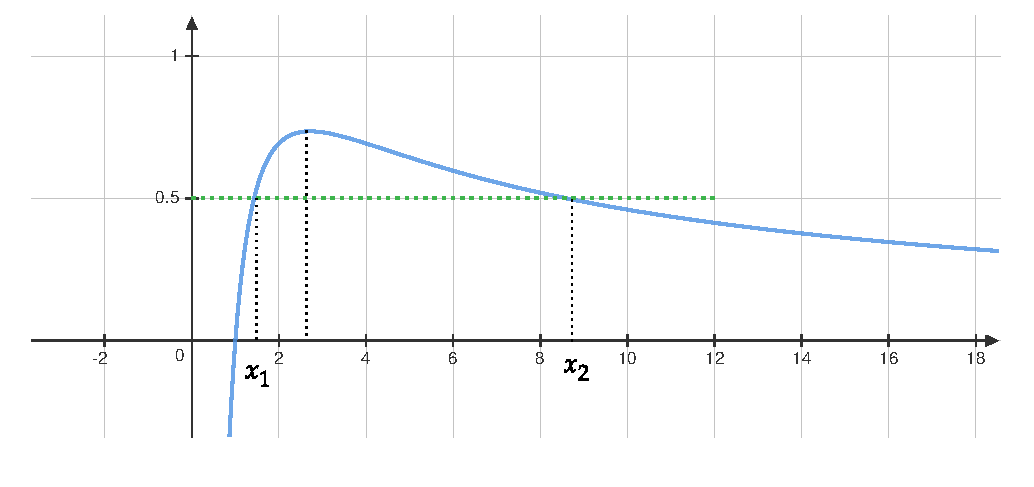
\includegraphics[scale=.6]{figures/diagram-20241127.pdf}
            \caption{}
        \end{figure}
    \end{enumerate}
\end{solution}

\subsection{不等式与函数凹凸性及拐点}

不等式与凸函数之间有着密切的关系, 凸函数在不等式中起着重要的作用.

\subsubsection{不等式}

\begin{theorem}[均值不等式]
    对任意 $n$ 个实数 $x_i\geqslant 0~~(i=1,2,\cdots,n)$, 有\label{meanInequality}
    调和平均数 $\leqslant$ 几何平均数 $\leqslant$ 算术平均数 $\leqslant$ 平方平均数, 即
    $$\begin{matrix}
            H_n                                                    & \leqslant & G_n                                                    & \leqslant & A_n       & \leqslant & Q_n       \\
            \parallel                                              &           & \parallel                                              &           & \parallel &           & \parallel \\
            \sqrt[n]{\displaystyle \sum_{i=1}^{n}\dfrac{1}{x_i}  } &           & \sqrt[n]{\displaystyle \prod _{i=1}^n x_i}             &           &
            \displaystyle \dfrac{1}{n}\sum_{i=1}^{n}x_i            &           & \sqrt{\displaystyle \dfrac{1}{n}\sum_{i=1}^{n}x_i^2  }
        \end{matrix}$$
    其中等号当且仅当 $a_1=a_2=\cdots=a_n$ 时成立.
    \index{均值不等式}
\end{theorem}

\begin{example}
    试比较 $\pi^{\mathrm{e}}$ 和 $\mathrm{e}^\pi$ 的大小, 并说明理由.
\end{example}
\begin{solution}
    \textbf{法一: }只需比较 $\dfrac{\ln \mathrm{e}}{\mathrm{e}}$ 与 $\dfrac{\ln\pi}{\pi}$ 的大小, 
    令 $f(x)=\dfrac{\ln x}{x}~~(x\geqslant \mathrm{e})\Rightarrow f'(x)=\dfrac{1-\ln x}{x^2}<0~~(x>\mathrm{e})$, 于是 $f(x)$ 在 $[\mathrm{e},+\infty)$ 上单调递减, 
    又 $\mathrm{e}<\pi$, 从而 $f(\pi)<f(\mathrm{e})$, 即 $\dfrac{\ln\pi}{\pi}<\dfrac{\ln \mathrm{e}}{\mathrm{e}}$, 故 $\mathrm{e}^\pi>\pi^{\mathrm{e}}.$\\
    \textbf{法二: }记 $\pi=\mathrm{e}+\lambda$, 则 $\lambda>0$, 于是
    $$\dfrac{\pi ^{\mathrm{e}}}{\mathrm{e}^{\pi }}=\dfrac{\left( \mathrm{e}+\lambda \right) ^{\mathrm{e}}}{\mathrm{e}^{\mathrm{e}+\lambda }}=\dfrac{1}{\mathrm{e}^{\lambda }}\left( \dfrac{\mathrm{e}+\lambda }{\mathrm{e}}\right) ^{\mathrm{e}}=\dfrac{1}{\mathrm{e}^{x}}\left[ \left( 1+\dfrac{\lambda }{\mathrm{e}}\right) ^{\dfrac{\mathrm{e}}{\lambda }}\right] ^{\lambda } <\dfrac{1}{\mathrm{e}^{\lambda }}\mathrm{e}^{\lambda }=1\Rightarrow\mathrm{e}^\pi>\pi^{\mathrm{e}}.$$
\end{solution}

\begin{example}[1995 数学 (二)]
    设 $ f(x) $ 二阶可导, 且 $ \displaystyle\lim _{x \to 0} \frac{f(x)}{x}=1,~f^{\prime \prime}(x)>0$, 
    证明 $ f(x) \geqslant x .$
\end{example}

\begin{proof}[{\songti \textbf{证法一}}]
    要证 $ f(x) \geqslant x$, 只需证 $ f(x)-x \geqslant 0$, 为此, 令 $ g(x)=f(x)-x$, 则由 $\displaystyle \lim _{x \to 0} \frac{f(x)}{x}=1$, 
    得 $$\displaystyle f(0)=\lim _{x \to 0} f(x)=0,~f^{\prime}(0)=\lim _{x \to 0} \frac{f(x)-f(0)}{x}=1$$ 
    所以 $$ g^{\prime}(x)=f^{\prime}(x)-1=f^{\prime}(x)-f^{\prime}(0)$$ 
    又由 $ f^{\prime \prime}(x)=\left(f^{\prime}(x)\right)^{\prime}>0 $ 知, $f^{\prime}(x)$  在 $ (-\infty,+\infty)$ 上单调递增, 
    于是当 $ x<0 $ 时, $g^{\prime}(x)<0$; 当 $ x>0 $ 时, $g^{\prime}(x)>0$, 从而知 $ x=0 $ 为 $ g(x) $ 的极小值点也是最小值点,, 
    故 $ g(x) \geqslant g(0)=0$, 即 $ f(x) \geqslant x .$
\end{proof}
\begin{proof}[{\songti \textbf{证法二}}]
    由 $\displaystyle \lim _{x \to 0} \frac{f(x)}{x}=1 $ 可知, $\displaystyle f(0)=\lim _{x \to 0} f(x)=0, f^{\prime}(0)=\lim _{x \to 0} \frac{f(x)-f(0)}{x}= \lim _{x \to 0} \frac{f(x)}{x}=1$, 
    由题设 $ f(x) $ 二阶可导, 将 $ f(x) $ 在 $ x=0 $ 点进行 Taylor 展开, 得
    $$f(x)=f(0)+f^{\prime}(0) x+\frac{f^{\prime \prime}(\xi)}{2 !} x^{2}$$
    其中 $ \xi $ 介于 $0$ 与 $ x $ 之间, 
    故由 $ f^{\prime \prime}(x)>0 $ 得 $ f(x) \geqslant f(0)+f^{\prime}(0) x=x $ (等号仅当 $ x=0 $ 时成立).
\end{proof}
\begin{proof}[{\songti \textbf{证法三}}]
    由 $\displaystyle \lim _{x \to 0} \frac{f(x)}{x}=1 $ 及 $ f(x) $ 连续可知, $\displaystyle f(0)=\lim _{x \to 0} f(x)=0, f^{\prime}(0)= \lim _{x \to 0} \frac{f(x)-f(0)}{x}=1$, 
    又由 $ f^{\prime \prime}(x)=\left(f^{\prime}(x)\right)^{\prime}>0 $ 知 $ f^{\prime}(x) $ 严格单调递增,  于是由 Lagrange 中值定理得\\
    当 $ x>0 $ 时, $\displaystyle\frac{f(x)}{x}=\frac{f(x)-f(0)}{x}=f^{\prime}\left(\xi_{1}\right)>f^{\prime}(0)=1$, 其中 $ \xi_{1} \in(0, x)$, 故 $ f(x)>x$; \\
    当 $ x<0 $ 时, $\displaystyle\frac{f(x)}{x}=\frac{f(x)-f(0)}{x}=f^{\prime}\left(\xi_{2}\right)<f^{\prime}(0)=1$, 其中 $ \xi_{2} \in(x, 0)$, 故 $ f(x)>x$; \\
    当 $ x=0 $ 时, $f(0)=0$, $\forall x \in(-\infty,+\infty)$, 都有 $ f(x) \geqslant x .$
\end{proof}

\begin{inference}
    一般地, 设 $\displaystyle\lim_{x\to0}\dfrac{f(x)}{x}=A$, 且 $f''(x)>0$, 则 $f(x)\geqslant Ax.$
\end{inference}

\begin{example}
    证明: $\qty|\dfrac{\sin x-\sin y}{x-y}-\cos y|\leqslant \dfrac{1}{2}\cdot |x-y|,~x\neq y.$
\end{example}
\begin{proof}[{\songti \textbf{证}}]
    将 $\sin x$ 在 $x=y$ 处 Taylor 展开, 得 $$\sin x=\sin y+\cos y(x-y)-\dfrac{1}{2}\sin \xi(x-y)^2$$
    其中 $\xi$ 介于 $x$ 与 $y$ 之间, 那么待证等式化简为 $$\qty|\dfrac{\sin x-\sin y}{x-y}-\cos y|=\qty|\dfrac{|\sin\xi|}{2}|~|x-y|$$
    又 $\sin \xi\leqslant 1$, 即得待证式成立.
\end{proof}

\begin{theorem}[Cauchy 不等式]
    设 $a_k,b_k$ 为任意实数 ($i=1,2,\cdots,n$), 则
    $$\displaystyle\left( \sum_{k=1}^n a_k b_k \right)^{\!\!2}\leqslant\left( \sum_{k=1}^n a_k^2 \right) \left( \sum_{k=1}^n b_k^2 \right) $$
    其中等号当且仅当 $a_k$ 与 $b_k$ 成比例时成立.
    \index{Cauchy 不等式}
\end{theorem}
% \begin{inference}
%     Carlson 不等式: $m\times n$ 的非负实数矩阵中, $n$ 列每列元素之和的几何平均值不小于矩阵中 $m$ 行每行元素的几何平均值之和. 即
%     $$\qty(x_1+y_1+\cdots)\qty(x_2+y_2+\cdots)\cdots\qty(x_n+y_n+\cdots)\geqslant \qty[\qty(\prod_{k=1}^{n}x_k)^{\frac{1}{n}}+\qty(\prod_{k=1}^{n}y_k)^{\frac{1}{n}}+\cdots]^n$$
%     等号成立的充要条件是至少有一列数都是 0 或所有行中的数对应成比例.
% \end{inference}

\subsubsection{凸函数的多种定义}

\begin{definition}[凸函数 A]
    设 $ f(x) $ 在区间 $ I $ 上有定义, $f(x) $ 在 $ I $ 上称为\textit{凸函数}, 当且仅当 $ \forall x_{1} ,  x_{2} \in I, \forall \lambda \in(0,1)$, 有
    $$f\left(\lambda x_{1}+(1-\lambda) x_{2}\right) \leqslant \lambda f\left(x_{1}\right)+(1-\lambda) f\left(x_{2}\right) .$$
    式中的 $\leqslant$ 改为 $<$ 便是严格凸的定义.
\end{definition}

\begin{definition}[凸函数 B]
    设 $ f(x) $ 在区间 $ I $ 上有定义, $f(x)$ 称为 $ I $ 上的凸函数, 当且仅当 $ \forall x_{1} ,  x_{2} \in I$, 有
    $$f\left(\frac{x_{1}+x_{2}}{2}\right) \leqslant \frac{f\left(x_{1}\right)+f\left(x_{2}\right)}{2} .$$
    式中的 $\leqslant$ 改为 $<$ 便是严格凸的定义.
\end{definition}

\begin{definition}[凸函数 C]
    设 $ f(x) $ 在区间 $ I $ 上有定义, $f(x) $ 称为凸函数, 当且仅当 $ \forall x_{1}, \cdots, x_{n} \in   I$, 有
    $$f\left(\frac{x_{1}+x_{2}+\cdots+x_{n}}{n}\right) \leqslant \frac{f\left(x_{1}\right)+f\left(x_{2}\right)+\cdots+f\left(x_{n}\right)}{n} .$$
    式中的 $\leqslant$ 改为 $<$ 便是严格凸的定义.
\end{definition}

\begin{definition}[凸函数 D]
    设 $ f(x) $ 在区间 $ I $ 上有定义, 当且仅当曲线 $ y=f(x) $ 的切线恒保持在曲线以下, 称 $ f(x) $ 为凸函数. 若除切点之外, 切线严格保持在曲线的下方, 则称 $ f(x) $ 为严格凸的.
\end{definition}

\begin{example}
    已知 $f(x)$ 为二阶导的正值函数, 且 $f(0)=f'(0)=1,~$, 则 (\quad).
    \begin{tasks}(2)
        \task $f(2)\leqslant \e^{2}\leqslant \sqrt{f(1)f(3)}$
        \task $\e^{2}\leqslant f(2)\leqslant \sqrt{f(1)f(3)}$
        \task $\sqrt{f(1)f(3)}\leqslant \e^{2}\leqslant f(2)$
        \task $\sqrt{f(1)f(3)}\leqslant f(2)\leqslant \e^{2}$
    \end{tasks}
\end{example}
\begin{solution}
    因为 $f(x)$ 为一正值函数, 且 $f(x)f''(x)\geqslant \qty[f'(x)]^2$, 于是有 $$\dfrac{f(x)f''(x)-\qty[f'(x)]^2}{f^2(x)}\geqslant 0\Rightarrow \qty(\dfrac{f'(x)}{f(x)})'\geqslant 0\Rightarrow \qty(\ln f(x))''\geqslant 0$$
    那么 $g(x)=\ln f(x)$ 为一下凸函数, 那么 $\dfrac{g(1)+g(3)}{2}=\dfrac{1}{2}\qty(\ln f(1)+\ln f(3))=\ln\sqrt{f(1)f(3)}$, 并且根据凸函数的性质, 有 $$\dfrac{g(1)+g(3)}{2}\geqslant g\qty(\dfrac{1+3}{2})=\ln f(2)\Rightarrow \ln\sqrt{f(1)f(3)}\geqslant \ln f(2)\Rightarrow f(2)\leqslant \sqrt{f(1)f(3)}$$
    将 $g(x)$在 $x=0$ 处 Taylor 展开, 得 $$g(x)=g(0)+g'(0)x+\dfrac{1}{2}g''(\theta)x^2\geqslant g(0)+g'(0)x=x$$
    于是得 $f(x)\geqslant \e^x$, 因此 $f(2)\geqslant \e^2$, 综上所述, 选 B.
\end{solution}

\begin{theorem}
    设函数 $ f(x) $ 在区间 $ I $ 上有定义, 则 $ f(x) $ 为凸函数的充要条件是: $ \forall x_{0} \in   r,~
        \exists  \alpha \text{, 使得 } \forall x \in I  \text{ 有 }  f(x) \geqslant \alpha\left(x-x_{0}\right)+f\left(x_{0}\right) .$
\end{theorem}

\begin{inference}
    设 $ f(x) $ 在区间 $ I $ 内部可导, 则 $ f(x) $ 在 $ I $ 上为凸的充要条件是: $ \forall x_{0} \in I^{\circ}$, 有
    $$f(x) \geqslant f^{\prime}\left(x_{0}\right)\left(x-x_{0}\right)+f\left(x_{0}\right)~ (\forall x \in I) .$$
\end{inference}

\begin{inference}
    若 $ f(x) $ 在区间 $ I $ 上为凸的, 则 $ \forall x_{0} \in I^{\circ}$, 在曲线 $ y=f(x) $ 上一点 $ \left(x_{0}\right. ,  \left.f\left(x_{0}\right)\right)$ 可作一条直线
    $$L: y=\alpha\left(x-x_{0}\right)+f\left(x_{0}\right)$$
    使曲线 $ y=f(x) $ 位于直线 $ L $ 上方.
\end{inference}

\begin{theorem}[分离性定理]
    若 $ f $ 为严格凸函数, 则除点 $ \left(x_{0}, f\left(x_{0}\right)\right) $ 之外曲线严格地在直线 $ L $ 的上方, 直线 $ L $ 称为 $ y=f(x) $ 的支撑.
    \index{分离性定理}
\end{theorem}

\begin{theorem}
    设 $ f(x) $ 在区间 $ I $ 上有导数, 则 $ f(x) $ 在 $ I $ 上为凸函数的充要条件是 $ f^{\prime}(x) \nearrow(x \in I) .$
\end{theorem}

\begin{theorem}[Jensen 不等式]
    若 $f(x)$ 在 $I$ 上有定义, 则
    $\forall q_{i} \geqslant 0$: $q_{1}+q_{2}+\cdots+q_{n}=1, \forall x_{1}, x_{2}, \cdots, x_{n} \in I$, 有
    $$f\left(q_{1} x_{1}+q_{2} x_{2}+\cdots+q_{n} x_{n}\right) \leqslant q_{1} f\left(x_{1}\right)+q_{2} f\left(x_{2}\right)+\cdots+q_{n} f\left(x_{n}\right);$$

    $\forall p_{i} \geqslant 0~ (i=1,2, \cdots, n)$ 不全为零, $\forall x_{1}, x_{2}, \cdots, x_{n} \in I$, 有
    $$f\left(\frac{p_{1} x_{1}+p_{2} x_{2}+\cdots+p_{n} x_{n}}{p_{1}+p_{2}+\cdots+p_{n}}\right) \leqslant \frac{p_{1} f\left(x_{1}\right)+p_{2} f\left(x_{2}\right)+\cdots+p_{n} f\left(x_{n}\right)}{p_{1}+p_{2}+\cdots+p_{n}} .$$
    \index{Jensen 不等式}
\end{theorem}

\begin{example}
    证明当 $0<x<\dfrac{\pi}{2}$ 时, $\sin x>\dfrac{2}{\pi}x.$
\end{example}
\begin{proof}[{\songti \textbf{证法一}}]
    设 $ f(x)=\sin x-\dfrac{2}{\pi} x$, 则 $$ f^{\prime}(x)=\cos x-\dfrac{2}{\pi}, f^{\prime \prime}(x)=-\sin x<0\left(0<x<\dfrac{\pi}{2}\right)$$ 于是
    $f(x) $ 在 $ \left[0, \dfrac{\pi}{2}\right] $ 上为凸函数, 又 $ f(0)=f\left(\dfrac{\pi}{2}\right)=0$, 故当 $ 0<x<\dfrac{\pi}{2} $ 时, $f(x)>0$, 即 $ \sin x>\dfrac{2}{\pi} x. $
\end{proof}
\begin{proof}[{\songti \textbf{证法二}}]
    设 $ f(x)=\sin x$, 则 $ f^{\prime}(x)=\cos x, f^{\prime \prime}(x)=-\sin x<0\left(0<x<\dfrac{\pi}{2}\right)$, 
    于是 $ f(x) $ 在 $ \left[0, \dfrac{\pi}{2}\right] $ 上是凸函数, 从而由凸函数的定义, 有
    $$f(x)=f\left[\dfrac{2 x}{\pi} \cdot \dfrac{\pi}{2}+\left(1-\dfrac{2 x}{\pi}\right) \cdot 0\right]>\dfrac{2 x}{\pi} \cdot f\left(\dfrac{\pi}{2}\right)+\left(1-\dfrac{2 x}{\pi}\right) \cdot f(0)=\dfrac{2 x}{\pi}$$
    即得 $ \sin x>\dfrac{2}{\pi} x\left(0<x<\dfrac{\pi}{2}\right) .$
\end{proof}
\begin{proof}[{\songti \textbf{证法三}}]
    设 $ f(x)=\sin x$, 对于 $ x \in\left(0, \dfrac{\pi}{2}\right)$, 将 $ f(t) $ 分别在 $ [0, x] $ 和 $ \left[x, \dfrac{\pi}{2}\right] $ 上应用 Lagrange 中值定理, 
    $$\exists\xi \in(0, x) \text{, 使得 }\dfrac{\sin x-\sin 0}{x-0}=\cos \xi$$
    即 $ \dfrac{\sin x}{x}=\cos \xi$, 
    又 $\exists\eta \in\left(x, \dfrac{\pi}{2}\right) \text{, 使得 }\dfrac{\sin \dfrac{\pi}{2}-\sin x}{\dfrac{\pi}{2}-x}=\cos \eta$, 
    即 $ \dfrac{1-\sin x}{\dfrac{\pi}{2}-x}=\cos \eta$, 
    又因为 $ \cos x $ 在 $ \left(0, \dfrac{\pi}{2}\right) $ 内严格单调递减, $\xi<\eta$, 所以 $ \cos \xi>\cos \eta$, 
    从而 $ \dfrac{\sin x}{x}>\dfrac{1-\sin x}{\dfrac{\pi}{2}-x}$, 即得 $ \sin x>\dfrac{2}{\pi} x\left(0<x<\dfrac{\pi}{2}\right) .$
\end{proof}

\subsubsection{拐点}

\begin{definition}[拐点]
    连续曲线凹与凸部分的分界点称为曲线的\textit{拐点}.\index{拐点}
\end{definition}

\begin{theorem}[拐点存在的必要条件]
    设函数 $f(x)$ 在点 $x_0$ 具有二阶导数, 则点 $(x_0,f(x_0))$ 是曲线 $y=f(x)$ 的拐点的必要条件是 $f''(x_0)=0.$
    \index{拐点存在的必要条件}
\end{theorem}

\begin{example}[2008 数二]
    求曲线 $y=(x-5)x^{\frac{2}{3}}$ 的拐点坐标.
\end{example}
\begin{solution}
    因为 $y'=\dfrac{5}{3}x^{\frac{2}{3}}-\dfrac{10}{3}x^{-\frac{1}{3}},~y''=\dfrac{10}{9}x^{-\frac{1}{3}}+\dfrac{10}{9}x^{-\frac{4}{3}}=\dfrac{10(x+1)}{9\sqrt[3]{x^4}}$, 显然 $y''(-1)=0,~y''(0)$ 不存在, 由 $y''$ 的表达式可知在 $x=-1$ 两侧 $y'$ 异号, 而 $x=0$ 两侧 $y'$ 不变号, 因此拐点坐标为 $(-1,-6).$
\end{solution}

\begin{example}[2018 数二]
    求曲线 $y=x^2+2\ln x$ 在其拐点处的切线方程.
\end{example}
\begin{solution}
    $y'=2x+\dfrac{2}{x},~y''=2-\dfrac{2}{x^2}$, 令 $y''=0\Rightarrow x=1~(\text{舍负})$, 拐点为 $(1,1)$, 切线的斜率为 $y'(1)=4$, 因此拐点处的切线方程为 $y=4x-3.$
\end{solution}

\begin{example}[2011 数二]
    设函数 $y=y(x)$ 由参数方程 $\begin{cases}
        x=\dfrac{1}{3}t^3+t+\dfrac{1}{3}\\[6pt]
        y=\dfrac{1}{3}t^3-t+\dfrac{1}{3}
    \end{cases}$ 确定, 求函数 $y=y(x)$ 的极值和曲线 $y=y(x)$ 的凹凸区间及拐点.
\end{example}
\begin{solution}
    由题意 $x'(t)=t^2+1,~x''(t)=2t,~y'(t)=t^2-1,~y''(t)=2t$, 则 
    $$\dv{y}{x}=\dfrac{y'(t)}{x'(t)}=\dfrac{t^2-1}{t^2+1},~\dv[2]{y}{x}=\dfrac{y''(t)x'(t)-x''(t)y'(t)}{x'^3(t)}=\dfrac{4t}{\qty(t^2+1)^3}$$
    令 $\displaystyle\dv{y}{x}=0\Rightarrow t=\pm 1$, 当 $t=1$ 时, $\displaystyle x=\dfrac{5}{3},~y=-\dfrac{1}{3},~\dv[2]{y}{x}>0$, 所以 $y=-\dfrac{1}{3}$ 为极小值, 
    当 $t=-1$ 时, $x=-1,~y=1,~\displaystyle\dv[2]{y}{x}<0$, 所以 $y=1$ 为极大值.\\
    令 $\displaystyle\dv[2]{y}{x}=0\Rightarrow t=0\Rightarrow x=y=\dfrac{1}{3}$, 当 $t<0$ 时, $x<\dfrac{1}{3},~\displaystyle \dv[2]{y}{x}<0$, 则曲线 $y=y(x)$ 在 $\qty(-\infty,\dfrac{1}{3})$ 上是凸的, 
    当 $t>0$ 时, $x>\dfrac{1}{3},~\displaystyle\dv[2]{y}{x}>0$, 则曲线 $y=y(x)$ 在 $\qty(-\infty,\dfrac{1}{3})$ 上是凹的, 点 $\qty(\dfrac{1}{3},\dfrac{1}{3})$ 是曲线的拐点.
\end{solution}

\subsection{导数的几何意义与曲线的曲率}

\subsubsection{导数的几何意义}

导数 $f'(x_0)$ 在几何上表示曲线 $y=f(x)$ 在点 $M(x_0,f(x_0))$ 处的切线斜率, 曲线 $y=f(x)$ 在点 $M$ 的切线方程为 $y=f'(x_0)(x-x_0)+f(x_0)$, 法线方程 $y=-\dfrac{1}{f'(x_0)}(x-x_0)+f(x_0)~~(f'(x_0)\neq 0).$

\begin{example}[2008 数一]
    求曲线 $\sin(xy)+\ln(y-x)=x$ 在点 $(0,1)$ 处的切线方程.
\end{example}
\begin{solution}
    等式 $\sin(xy)+\ln(y-x)=x$ 两端对 $x$ 求导, 得 $\cos(xy)\qty(y+xy')+\dfrac{y'-1}{y-x}=1$, 并令 $x=0,~y=1$, 解得 $y'(0)=1$, 于是该曲线在点 $(0,1)$ 处的切线方程为 $y=x+1.$
\end{solution}

\begin{example}[2010 数二]
    曲线 $y=x^2$ 与曲线 $y=a\ln x~(a\neq 0)$ 相切, 则 $a$ 等于 (\quad).
    \begin{tasks}(4)
        \task $4\e$
        \task $3\e$
        \task $2\e$
        \task $\e$
    \end{tasks}
\end{example}
\begin{solution}
    设曲线 $y=x^2$ 与曲线 $y=a\ln x~(a\neq 0)$ 的公切点为 $(x_0,y_0)$, 则 $\begin{cases}
            x_0^2=a\ln x_0 \\2x_0=\dfrac{a}{x_0}
        \end{cases}$, 解得 $x_0=\sqrt{\e}$, 那么 $a=2\e$, 故选 C.
\end{solution}

\begin{example}
    求对数螺线 $r=\e^\theta$ 在 $(r,\theta)=\qty(\e ^{\frac{\pi}{2}},\dfrac{\pi}{2})$ 处的切线的直角坐标方程.
\end{example}
\begin{solution}
    由图 \ref{archimedesSpiral} 知对数螺线的参数方程为 $\begin{cases}
        x=\e^\theta\cos\theta\\y=\e^\theta\sin\theta
    \end{cases}$ 那么 
    $$\eval{\dv{y}{x}}_{\theta=\frac{\pi}{2}}=\eval{\dfrac{\dd y/\dd \theta}{\dd x/\dd \theta}}_{\theta=\frac{\pi}{2}}=\eval{\dfrac{\sin\theta+\cos\theta}{\cos\theta-\sin\theta}}_{\theta=\frac{\pi}{2}}=-1$$
    因此在 $(r,\theta)=\qty(\e ^{\frac{\pi}{2}},\dfrac{\pi}{2})\Rightarrow (x,y)=\qty(0,\e ^{\frac{\pi}{2}})$ 处的切线的直角坐标方程为 $x+y=\e ^{\frac{\pi}{2}}.$
\end{solution}

\begin{example}
    已知 $f(x)$ 是周期为 5 的连续函数, 它在 $x=0$ 的某邻域内满足关系式 $$
    f(1+\sin x)-3f(1-\sin x)=8x+\alpha(x)
    $$
    其中 $\alpha(x)$ 是当 $x\to 0$ 时比 $x$ 的高阶无穷小, 且 $f(x)$ 在 $x=1$ 处可导, 求曲线 $y=f(x)$ 在点 $(6,f(6))$ 处的切线方程.
\end{example}
\begin{solution}
    由题意得 $\displaystyle \lim_{x \to 0}[f(1+\sin x)-3f(1-\sin x)]=\lim_{x \to 0}(8x+\alpha(x))\Rightarrow f(1)=0$, 由导数定义得 
    $$
    \lim_{x \to 0}\dfrac{f(1+\sin x)-3f(1-\sin x)}{\sin x}\xlongequal{t=\sin x}\lim_{t \to 0}\qty[\dfrac{f(1+t)-f(1)}{t}+3\dfrac{f(1)-f(1-t)}{t}]=4f'(1)=\lim_{x \to 0}\dfrac{8x+\alpha(x)}{\sin x}=8
    $$
    因此 $f'(1)=2$, 又 $T=5$, 所以 $f'(6)=f'(1)=2,f(6)=f(1)=0$, 故在点 $(6,f(6))$ 处的切线方程为 $y=2x-12.$
\end{solution}

\subsubsection{曲线的曲率}

\begin{definition}[曲率]
    在曲线 $L$ 上, 点 $N$ 沿曲线 $L$ 趋于点 $M$ 时, 如果极限 $\displaystyle\lim_{\Delta s\to0}\bar{K}=\lim_{\Delta s\to0}\qty|\dfrac{\Delta\alpha}{\Delta s}|$ 存在, 则称此极限值为曲线 $L$ 在点 $M$ 处的\textit{曲率}, 记作 $K=\displaystyle\lim_{\Delta s\to0}\qty|\dfrac{\Delta\alpha}{\Delta s}|$.
    在 $\displaystyle\lim_{\Delta s\to0}\dfrac{\Delta\alpha}{\delta s}=\dv{\alpha}{s}$ 存在的条件下, $K$ 也可以表示为 $K=\qty|\dfrac{\dd \alpha}{\dd s}|$. ($\Delta \alpha$ 为动点 $N$ 移动到 $M$ 时切线转过的角度, $\Delta s$ 为弧段 $\widehat{NM} $ 的长度).
    \index{曲率}
\end{definition}

\begin{theorem}[曲率的计算公式]\index{曲率的计算公式}
    设曲线的直角坐标方程是 $y=f(x)$, 且 $f(x)$ 具有二阶导数, 则曲率公式为 $$K=\dfrac{|y''|}{\qty(1+\qty(y')^2)^{3/2}}$$
    若曲线方程由参数方程 $\begin{cases}
            x=\varphi(t) \\y=\psi(t)
        \end{cases}(\alpha \leqslant t\leqslant \beta)$ 给出, 则可利用参数方程确定的函数的求导法, 求出 $y_x'$ 及 $y''_x$ 代入曲率公式即可, 或者代入以下公式
        $$
        K=\dfrac{|y''x'-x''y'|}{\qty[\qty(x')^2+\qty(y')^2]^{3/2}}.
        $$
\end{theorem}

\begin{example}[2012 数二]
    求曲线 $y=x^2+x~(x<0)$ 上曲率为 $\dfrac{\sqrt{2}}{2}$ 的点的坐标.
\end{example}
\begin{solution}
    $y'=2x+1,~y''=2$, 那么 $K=\dfrac{|y''|}{\qty(1+y'^2)^{3/2}}=\dfrac{\sqrt{2}}{2}\Rightarrow (2x+1)^2=1\Rightarrow x=0,-1$, 又 $x<0$, 故坐标为 $(-1,0).$
\end{solution}

\begin{example}[2018 数二]
    求曲线 $\begin{cases}
            x=\cos^3t \\y=\sin^3t
        \end{cases}$ 在 $t=\dfrac{\pi}{4}$ 对应点处的曲率.
\end{example}
\begin{solution}
    \textbf{法一: }求出各分量代入曲率公式 $K=\dfrac{|y''x'-x''y'|}{\qty[\qty(x')^2+\qty(y')^2]^{3/2}}$, 
    \begin{flalign*}
        x'\qty(\dfrac{\pi}{4}) & =\eval{-3\cos^2t\sin t}_{t=\frac{\pi}{4}}=-\dfrac{3\sqrt{2}}{4},~x''\qty(\dfrac{\pi}{4})  =\eval{6\cos t\sin^2t-3\cos^3t}_{t=\frac{\pi}{4}}=\dfrac{3\sqrt{2}}{4} \\
        y'\qty(\dfrac{\pi}{4}) & =\eval{3\sin^2\cos t}_{t=\frac{\pi}{4}}=\dfrac{3\sqrt{2}}{4},~y''\qty(\dfrac{\pi}{4})  =\eval{6\sin t\cos^2t-3\sin^3t}_{t=\frac{\pi}{4}}=\dfrac{3\sqrt{2}}{4}
    \end{flalign*}
    于是 $K=\dfrac{2}{3}.$\\
    \textbf{法二: }$\displaystyle \dv{y}{x}=\dv{y}{t}\qty(\dv{x}{t})^{-1}=-\tan t,~\dv[2]{y}{x}=\dfrac{1}{3\cos ^4t\sin t}$, 于是 $K=\eval{\dfrac{|y''|}{\qty(1+\qty(y')^2)^{3/2}}}_{t=\frac{\pi}{4}}=\dfrac{2}{3}.$
\end{solution}

\begin{example}
    设 $y=y(x)$ 是由方程 $2y^3-2y^2+2xy-x^2=1$ 确定, 求 $y=y(x)$ 的极值, 并求极值点处的曲率圆方程.
\end{example}
\begin{solution}
    方程两边对 $x$ 求导得 $$
    6y^2\cdot y'-4y\cdot y'+2y+2xy'-2x=0\Rightarrow y'=\dfrac{x-y}{x-2y+3y^2}
    $$
    令 $y'=0$ 得 $x=y$, 代入方程求得驻点 $x=1$, 并且 
    $$
    12y\cdot y'^2+6y^2\cdot y''-4y'^2-4y\cdot y''+4y'+2x\cdot y''-2=0
    $$
    代入 $x=y=1,y'(1)=0$ 得 $y''(1)=\dfrac{1}{2}$, 因此 $y(1)=1$ 为极小值, 曲线在 $(1,1)$ 处的曲率为 $$
    K=\dfrac{|y''|}{\qty(1+y'^2)^{\frac{3}{2}}}=\dfrac{1}{2}
    $$
    故曲率圆半径 $R=\dfrac{1}{K}=2$, 点 $(1,1)$ 处的法线方程为 $x=1$, 又 $y''(1)=\dfrac{1}{2}>0$, 所以曲率圆的圆心坐标为 $(1,3)$, 故曲率圆方程为 $(x-1)^2+(y-3)^2=4.$
\end{solution}

\subsection{导数不等式证明中的应用}

\begin{example}
    设 $\qty{a_n}$ 为常数列, 且 $\displaystyle\qty|\sum_{k=1}^{n}a_k\sin(kx)|\leqslant |\sin x|,~\qty|\sum_{k=1}^{n}a_{n-k+1}\sin(kx)|\leqslant |\sin x|$, 证明: $$\displaystyle \qty|\sum_{k=1}^{n}a_k|\leqslant \dfrac{2}{n+1}.$$
\end{example}
\begin{proof}[{\songti \textbf{证}}]
    分别令 $\displaystyle f(x)=\sum_{k=1}^{n}a_k\sin(kx),~g(x)=\sum_{k=1}^{n}a_{n-k+1}\sin(kx)$, 则 $f,g$ 在定义域内连续, 且 $f(0)=g(0)=0$, 于是
    $$f'(x)=\sum_{k=1}^{n}ka_k\cos kx,~g'(x)=\sum_{k=1}^{n}ka_{n-k+1}\cos kx$$
    由 Lagrange 中值定理知, $\exists\xi_1,\xi_2\in(0,x)$, 使得
    $$f(x)-f(0)=f'(\xi_1)x\Rightarrow f(x)=f'(\xi_1)x,~g(x)-g(0)=g'(\xi_2)x\Rightarrow g(x)=g'(\xi_2)x$$
    因此 $f'(\xi_1)+g'(\xi_2)=\dfrac{f(x)}{x}+\dfrac{g(x)}{x}$, 一方面
    $$\qty|f'(\xi_1)+g'(\xi_2)|=\qty|\dfrac{f(x)}{x}+\dfrac{g(x)}{x}|\leqslant \qty|\dfrac{f(x)}{x}|+\qty|\dfrac{g(x)}{x}|\leqslant 2\qty|\dfrac{\sin x}{x}|\to 2~~(x\to0)$$
    另一方面当 $x\to0$ 时, $\xi_1,\xi_2\to0$, 则
    $$\qty|f'(0)+g'(0)|\to\qty|\sum_{k=1}^{n}ka_k+\sum_{k=1}^{n}ka_{n-k+1}|=\qty|\sum_{k=1}^{n}ka_k+\sum_{k=1}^{n}(n-k+1)a_k|=\qty|\sum_{k=1}^{n}\qty[k+(n-k+1)]a_k|=(n+1)\qty|\sum_{k=1}^{n}a_k|$$
    所以, 当 $x\to0$ 时, 有 $\displaystyle (n+1)\qty|\sum_{k=1}^{n}a_k|\leqslant 2\Rightarrow \qty|\sum_{k=1}^{n}a_k|\leqslant \dfrac{2}{n+1}.$
\end{proof}
